%&preamble
% automatic hyphenation for 2 languages
% http://www.mechpedia.gr/wiki/Hyphenation_-_%CE%A5%CF%86%CE%B5%CE%BD%CF%8E%CF%83%CE%B5%CE%B9%CF%82#.CE.91.CF.85.CF.84.CF.8C.CE.BC.CE.B1.CF.84.CE.B5.CF.82_.CF.85.CF.86.CE.B5.CE.BD.CF.8E.CF.83.CE.B5.CE.B9.CF.82_.CF.83.CE.B5_.CE.B4.CE.AF.CE.B3.CE.BB.CF.89.CF.83.CF.83.CE.B1_.CE.BA.CE.B5.CE.AF.CE.BC.CE.B5.CE.BD.CE.B1
% very slow, enable only at final pdf.
\usepackage[Greek,Latin]{ucharclasses}
\setTransitionsForGreek{\selectlanguage{greek}}{\selectlanguage{english}}

% polyglossia
\usepackage{polyglossia}
\setmainlanguage{greek}
\setotherlanguages{english}

% Fonts
% fonts can't go in the .fmt file
\usepackage{fontspec}
\setmainfont[Mapping=tex-text]{DejaVu Sans}
\newfontfamily\greekfont[Script=Greek]{DejaVu Sans}
\newfontfamily\greekfontsf[Script=Greek]{DejaVu Sans}
\setmonofont[Scale=1.0]{Source Code Pro Medium}
\newfontfamily\greekfonttt[Scale=1.0]{Source Code Pro Medium}
\usepackage{microtype} % microtype is font-dependant


\title{CellLock}

\author{%
  Ομάδα Daedalus:\\
  Παπουδάκης Γεώργιος \href{mailto:papoudak@ece.auth.gr}{papoudakis@ece.auth.gr} \\
  Φλώρος-Μαλιβίτσης Ορέστης \href{mailto:orestisf@ece.auth.gr}{orestisf@ece.auth.gr}\\
  Χαμζάς Κωνσταντίνος \href{mailto:chamzask@gmail.com}{chamzask@gmail.com} \\
  Κίρτσιος Δημήτριος \href{mailto:dimkirt@hotmail.com}{dimkirt@hotmail.com} \\
  Τσιριγώτης Χρήστος \href{mailto:tsirif@gmail.com}{tsirif@gmail.com} \\
  \\\\
  \textbf{Τμήμα Ηλ. Μηχανικών / Μηχανικών ΗΥ}\\
  \textbf{Αριστοτέλειο Πανεπιστήμιο Θεσσαλονίκης}
}

\titlepic{
\includegraphics[width=0.40\textwidth]{images/logo}}

\newcommand{\imageref}[1] {%
\hyperref[fig:#1]{\figurename{} \ref{fig:#1}}}
\newcommand{\imagerefc}[2] {%
\hyperref[fig:#1]{fig:#2}}

\begin{document}
\maketitle
\section{Περιγραφή της εφαρμογής}
Το CellLock είναι μια εφαρμογή που στοχεύει στην προστασία του κινητού σας από κλοπή ή απώλεια.

Μετά από την σύνδεση του κινητού σας με το κύκλωμα μέσω bluetooth, σας δίνεται η δυνατότητα να μπείτε στην λειτουργία "protection".
Σε αυτή τη φάση όταν το κινητό βρεθεί σε μεγαλύτερη από την προκαθορισμένη απόσταση από το κύκλωμα (λειτουργία "danger") ενεργοποιείται ένας συναγερμός τόσο στο κινητό, που απαιτεί έναν κωδικό πρόσβασης για να απενεργοποιηθεί, όσο και στο κύκλωμα.
Με αυτό τον τρόπο ειδοποιείται ο κάτοχος του κινητού για την απώλεια του.

Επίσης, δίνεται η δυνατότητα στον χρήστη να αναζητήσει το κινητό του πατώντας ένα κουμπί πάνω στο κύκλωμα που στέλνει μήνυμα \texttt{"RING"} στην συνδεδεμένη εφαρμογή του κινητού. Αυτό, προκαλεί την αναπαραγωγή του συναγερμού και σκοπεύει στην εύρεση του κινητού αν αυτό έχει χαθεί. Αντίστοιχη λειτουργία υπάρχει και από την πλευρά του κινητού για την εύρεση του κυκλώματος. Κάτι τέτοιο βοηθάει πχ αν ο χρήστης τοποθετήσει το κύκλωμα στα κλειδιά του και μετά τα χάσει.

\subsection{Περιγραφή hardware \& κώδικα arduino}
\renewcommand{\figurename}{Σχήμα}
\begin{figure}[htb]
    \centering
    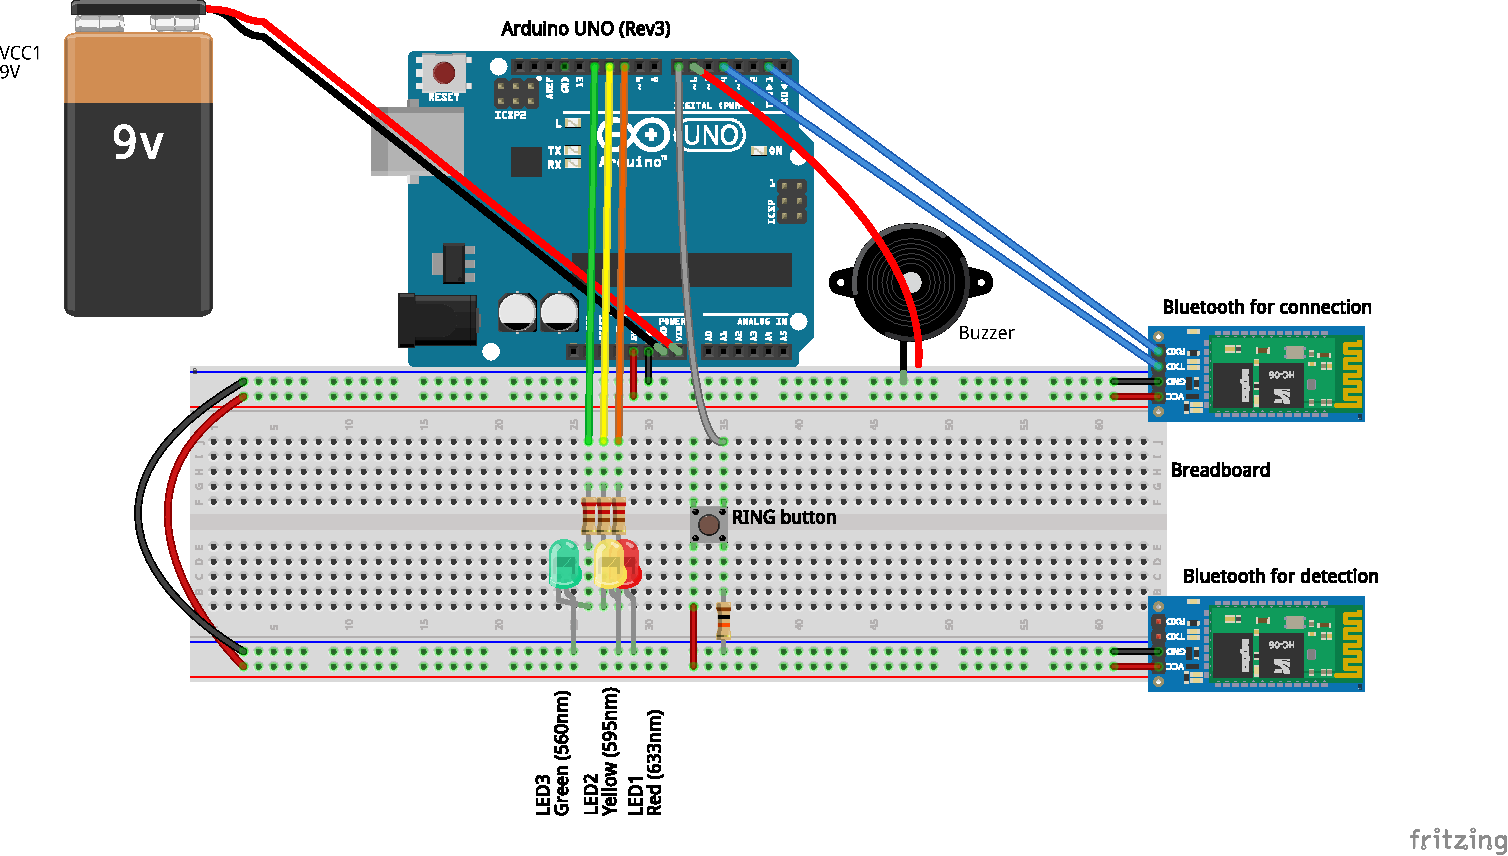
\includegraphics[keepaspectratio, width=\linewidth]{hardware/sketch_bb}
    \caption{Το κύκλωμα που χρησιμοποιήθηκε}
    \label{fig:hardware}
\end{figure}
Από πλευρά hardware χρησιμοποιήθηκαν:
\begin{itemize}
\item 1 \href{https://www.arduino.cc/en/Main/ArduinoBoardUno}{Arduino UNO Rev3}
\item 2 HC06 - Bluetooth Module for Arduino
\item 1 breadboard
\item 3 LEDάκια
\item 1 μπαταρία \SI{9}{\volt} με έναν \href{http://playground.arduino.cc/Learning/9VBatteryAdapter}{9V battery adapter} για arduino.
\item 1 buzzer.
\item 1 κομπί.
\item Καλώδια και αντιστάσεις.
\end{itemize}

Στο arduino εκτελούνται όλες οι βασικές λειτουργίες.
Ο κυρίως κώδικας βρίσκεται στο αρχείο \url{Arduino/daerduino/daerduino.ino}:
\begin{itemize}
\item \sloppy Η συνάρτηση \lstinline[language=C++]!bool emergencyButtonPressed()! εκτελείται σε κάθε επανάληψη της κύριας \lstinline[language=C++]!loop()! και αν ανιχνεύσει συνεχόμενο πάτημα του κουμπιού επί τουλάχιστον 1 δευτερόλεπτο επιστρέφει \lstinline[language=C++]!true!.

\item Η συνάρτηση \lstinline[language=C++]!String readBT()! διαβάζει χαρακτήρες από το bluetooth μέχρι να συναντήσει τον χαρακτήρα \lstinline[language=C++]!';'!.

\item \sloppy Η συνάρτηση \lstinline[language=C++]!void interruptBluetooth()! καλείται σαν timer interrupt
κάθε \lstinline[language=C++]!INTERRUPT_FREQUENCY_MICROS! \si{\micro\second}
και στέλνει στη συνδεδεμένη συσκευή android τον χαρακτήρα \lstinline[language=C++]!"C"! ώστε να επιβεβαιωθεί η σύνδεση και διαβάζει τις εντολές που στέλνει η συσκευή android.
Οι διαθέσιμες εντολές είναι:
\begin{itemize}
\item \lstinline[language=C++]!"RING"!: ενεργοποιεί το alarm: \lstinline[language=C++]!playRing = true;!.
\item \lstinline[language=C++]!"RSTOP"!: απενεργοποιεί το alarm: \lstinline[language=C++]!playRing = false;!.
\item \lstinline[language=C++]!"POFF"!: απενεργοποίηση προστασίας.
\item \lstinline[language=C++]!"PON"!: κατάσταση προστασίας.
\item \lstinline[language=C++]!"SEMI"!: κατάσταση ημι-κινδύνου.
\item \lstinline[language=C++]!"DANG"!: κατάσταση κινδύνου.
\end{itemize}

\item Η συνάρτηση \lstinline[language=C++]!void updateLEDs()! διαχειρίζεται τα LEDs ανάλογα με την τρέχουσα κατάσταση.

\item Η συνάρτηση \lstinline[language=C++]!void updateLEDs()! διαχειρίζεται τα LEDs ανάλογα με την τρέχουσα κατάσταση.

\item Η συνάρτηση \lstinline[language=C++]!void loop()! είναι η κυρίως λούπα της εφαρμογής, αναλαμβάνει:
\begin{itemize}
\item Το reset του watchdog.
\item Την αναπαραγωγή του alarm μέσω της \lstinline[language=C++]!sing()! εάν η \lstinline[language=C++]!alarmShouldPlay()! επιστρέψει \lstinline[language=C++]!true!.
\item Την αποστολή της εντολής \lstinline[language=C++]!"RING"! στην συσκευή android σύμφωνα με την επιστρεφόμενη τιμή της \lstinline[language=C++]!emergencyButtonPressed()!.
\end{itemize}
\end{itemize}

Στο \url{Arduino/daerduino/supermario.ino}
βρίσκεται η συνάρτηση \lstinline[language=C++]!sing()! που αναλαμβάνει την αναπαραγωγή του alarm στο buzzer.

\section{Περιγραφή του android app}
% Backup original figurename command to restore later.
\let\originalfigurename\figurename
% Set figurename command.
\renewcommand{\figurename}{Εικόνα}
\newcommand{\screenshot}[2]{%
\begin{figure}[H]
\centering%
\maxsizebox{\linewidth}{0.3\textheight}{\includegraphics[keepaspectratio]{screenshots/#1}}%
\caption{#2}%
\label{fig:#1}%
\end{figure}%
}

\screenshot{bluetooth-open}{Ερώτηση για άνοιγμα bluetooth}
\screenshot{not-connected}{Κατάσταση χωρίς σύνδεση με τα bluetooth του κυκλώματος}
\screenshot{not-protected}{Κατάσταση χωρίς προστασία}
\screenshot{protected}{Κατάσταση με προστασία}
\screenshot{ring}{Κατάσταση αναπαραγωγής ήχου για την εύρεση της συσκευής}

\FloatBarrier
Για την ανάπτυξη της εφαρμογής μας χρησιμοποιήθηκε το android studio και το αντίστοιχο API για Bluetooth.
Παρακάτω υπάρχουν κάποια επιμέρους ζητήματα που αναλύονται περισσότερο.

\subsection{Ισχύς Ζεύξης Συσκευών}
Βασική απαίτηση της εφαρμογής μας ήταν να έχει την δυνατότητα εκτίμησης της απόστασης.
Το API του Android όμως δεν δίνει την τιμή RSSI (Received Signal Strength Indication) όταν είναι συνδεδεμένο ένα κινητό με ένα bluetooth.
Η τιμή του rssi δίνεται μόνο κατά την διαδικασία της αναζήτησης συσκευών (discovery) κατά την οποία όμως δεν μπορούμε να βρούμε συσκευές με τις οποίες ήμαστε ήδη συνδεδεμένοι.
Συνεπώς, χρησιμοποιήθηκαν 2 bluetooth στην εφαρμογή μας: ένα για discovery και ένα για connection.

Για να μπορούμε να μετρήσουμε την απόσταση των δύο συσκευών μας, είναι
απαραίτητο να γνωρίζουμε την ισχύ της ζεύξης των δύο συσκευών.
Το API του android μας επιστρέφει την τιμή του rssi σε dB με τον τρόπο που αναφέρθηκε.

Μέσα από διάφορα πειράματα που εκτελέστηκαν κατά την διάρκεια του διαγωνισμού
φτάσαμε στα παρακάτω συμπεράσματα:
\begin{itemize}
\item Η απόσταση στην οποία πρέπει να ενεργοποιείται ο κίνδυνος είναι 5 με 6
μέτρα.
\item Σε απόσταση 4 με 5 μέτρα πρέπει να βρισκόμαστε στην κατάσταση στην οποία
υπάρχει προειδοποίηση για πιθανό κίνδυνο.
\end{itemize}

Οπότε, καταλήξαμε πως για τιμές του rssi μεγαλύτερες από -75dB βρισκόμαστε σε
ασφαλή κατάσταση.
Για τιμές μεταξύ -75dB και -80dB βρισκόμαστε σε κατάσταση πιθανού
κινδύνου, ενώ σε τιμές μικρότερες από -80dB σε κατάσταση κινδύνου.

\subsection{Λογική του Προγράμματος}
Επειδή η εφαρμογή μας πρέπει να λειτουργεί με κάποιου είδους μνήμη στις εισόδους που δέχεται (πάτημα κουμπιών, ισχύς σήματος) χρησιμοποιήθηκε η λογική των states για να δομηθεί το πρόγραμμά μας.
Τα states καθώς και οι μεταβάσεις φαίνονται στο
\renewcommand{\figurename}{Σχήμα}
\hyperref[fig:stdiag]{\figurename{} \ref{fig:stdiag}}.
\begin{figure}[htb]
    \centering
    \includegraphics[keepaspectratio, width=\linewidth]{images/state-diagram}
    \caption{Το διάγραμμα καταστάσεων}
    \label{fig:stdiag}
\end{figure}

\end{document}
